%%%%%%%%%%%%%%%%%%%%%%%%%%%%%%%%%%%%%%%%%
% Beamer Presentation
% LaTeX Template
% Version 1.0 (10/11/12)
%
% This template has been downloaded from:
% http://www.LaTeXTemplates.com
%
% License:
% CC BY-NC-SA 3.0 (http://creativecommons.org/licenses/by-nc-sa/3.0/)
%
%%%%%%%%%%%%%%%%%%%%%%%%%%%%%%%%%%%%%%%%%

%----------------------------------------------------------------------------------------
%	PACKAGES AND THEMES
%----------------------------------------------------------------------------------------

\documentclass{beamer}

\mode<presentation> {

% The Beamer class comes with a number of default slide themes
% which change the colors and layouts of slides. Below this is a list
% of all the themes, uncomment each in turn to see what they look like.

%\usetheme{default}
%\usetheme{AnnArbor}
%\usetheme{Antibes}
%\usetheme{Bergen}
%\usetheme{Berkeley}
%\usetheme{Berlin}
%\usetheme{Boadilla}
%\usetheme{CambridgeUS}
%\usetheme{Copenhagen}
%\usetheme{Darmstadt}
%\usetheme{Dresden}
%\usetheme{Frankfurt}
%\usetheme{Goettingen}
%\usetheme{Hannover}
%\usetheme{Ilmenau}
%\usetheme{JuanLesPins}
%\usetheme{Luebeck}
%\usetheme{Madrid}
%\usetheme{Malmoe}
%\usetheme{Marburg}
%\usetheme{Montpellier}
%\usetheme{PaloAlto}
%\usetheme{Pittsburgh}
%\usetheme{Rochester}
%\usetheme{Singapore}
%\usetheme{Szeged}
\usetheme{Warsaw}
%\beamertemplatenavigationsymbolsempty

% As well as themes, the Beamer class has a number of color themes
% for any slide theme. Uncomment each of these in turn to see how it
% changes the colors of your current slide theme.

%\usecolortheme{albatross}
%\usecolortheme{beaver}
%\usecolortheme{beetle}
%\usecolortheme{crane}
%\usecolortheme{dolphin}
%\usecolortheme{dove}
%\usecolortheme{fly}
%\usecolortheme{lily}
%\usecolortheme{orchid}
%\usecolortheme{rose}
%\usecolortheme{seagull}
%\usecolortheme{seahorse}
%\usecolortheme{whale}
%\usecolortheme{wolverine}

%\setbeamertemplate{footline} % To remove the footer line in all slides uncomment this line
%\setbeamertemplate{footline}[page number] % To replace the footer line in all slides with a simple slide count uncomment this line

%\setbeamertemplate{navigation symbols}{} % To remove the navigation symbols from the bottom of all slides uncomment this line
}

\usepackage{graphicx} % Allows including images
\usepackage{booktabs} % Allows the use of \toprule, \midrule and \bottomrule in tables
%\usepackage{etex}
\usepackage[T1]{fontenc}
\usepackage[utf8]{inputenc}
\usepackage[english]{babel}
\usepackage{cite}
\usepackage{amsmath,amsfonts,amssymb,amsthm}
\usepackage{mathrsfs,mathtools}
\usepackage{graphicx}
\usepackage{float}

\usepackage{hyperref} % References become hyperlinks.
\hypersetup{
	%colorlinks = true,
	linkcolor = {blue},
	urlcolor = {red},
	citecolor = {blue},
	%pdfenconing=auto,
}
\usepackage{wrapfig}
%\usepackage{arydshln}
\usepackage{array}
\usepackage[T1]{fontenc} 
\usepackage{bm}
\usepackage{multicol, multirow}
\usepackage{grffile,pgf,tikz}
\usepackage{verbatim}
\usepackage{graphicx}
\usepackage{animate}
\usepackage{caption}
\usepackage{subcaption}

% Default fixed font does not support bold face
\DeclareFixedFont{\ttb}{T1}{txtt}{bx}{n}{12} % for bold
\DeclareFixedFont{\ttm}{T1}{txtt}{m}{n}{12}  % for normal

% Custom colors
\usepackage{color}
\definecolor{deepblue}{rgb}{0,0,0.5}
\definecolor{deepred}{rgb}{0.6,0,0}
\definecolor{deepgreen}{rgb}{0,0.5,0}

\usepackage{listings}

% Python style for highlighting
\newcommand\pythonstyle{\lstset{
		language=Python,
		basicstyle=\ttm,
		morekeywords={self},              % Add keywords here
		keywordstyle=\ttb\color{deepblue},
		emph={MyClass,__init__},          % Custom highlighting
		emphstyle=\ttb\color{deepred},    % Custom highlighting style
		stringstyle=\color{deepgreen},
		frame=tb,                         % Any extra options here
		showstringspaces=false
}}


% Python environment
\lstnewenvironment{python}[1][]
{
	\pythonstyle
	\lstset{#1}
}
{}

% Python for external files
\newcommand\pythonexternal[2][]{{
		\pythonstyle
		\lstinputlisting[#1]{#2}}}

% Python for inline
\newcommand\pythoninline[1]{{\pythonstyle\lstinline!#1!}}



\usetikzlibrary{matrix}
\usetikzlibrary{shapes.geometric,calc,arrows}

%\usepackage{unicode-math}
%\setmathfont{XITS Math}
%\setmathfont[version=setB,StylisticSet=1]{XITS Math}


\theoremstyle{plain}
\newtheorem{teo}{Teorema}
%\newtheorem{lemma}[teo]{Lemma}
\newtheorem{prop}[teo]{Proposizione}
\newtheorem{post}{Postulato}
\newtheorem{cor}[teo]{Corollario}


\theoremstyle{definition}
\newtheorem{defn}{Definizione}
\newtheorem{exmp}[defn]{Esempio}
\newtheorem{oss}[defn]{Osservazione}
\newtheorem{prob}{Problema}
\newtheorem*{prob*}{Problema}
\newtheorem{hint}{Indizio}
\newtheorem*{notaz}{Notazione}

\theoremstyle{remark}
\newtheorem*{rem}{Remark}


\newcommand{\C}{\mathbb{C}}
\newcommand{\R}{\mathbb{R}}
\newcommand{\K}{\mathbb{K}}
\newcommand{\Q}{\mathbb{Q}}
\newcommand{\Z}{\mathbb{Z}}
\newcommand{\N}{\mathbb{N}}
\newcommand{\M}{\mathbb{M}}
\newcommand{\LL}{\mathscr{L}}
\newcommand{\HH}{\mathbb{H}}
\newcommand{\SP}{\mathbb{S}}
\newcommand{\dsum}{\displaystyle\sum}
\newcommand{\dint}{\displaystyle\int}
\newcommand{\scal}[2]{\langle #1,#2 \rangle}
\newcommand{\norm}[1]{\lVert#1\rVert}
\newcommand{\eval}[3]{\Big[ #1 \Big]_{#2}^{#3}}
%\newcommand{\sob}[3]{W^{#1, #2}(#3)}
%\newcommand{\sobzero}[3]{W_{0}^{#1, #2}(#3)}
%\newcommand{\sobloc}[3]{W_{\text{loc}}^{#1, #2}(#3)}
\newcommand{\weakconv}{\rightharpoonup}
\newcommand{\weakconvs}{\overset{\ast}{\rightharpoonup}}
\newcommand{\prox}{\text{prox}}


\newcommand{\dx}{\text{d}x}
\newcommand{\dt}{\text{d}t}
\newcommand{\dy}{\text{d}y}
\newcommand{\diff}{\text{d}}
\newcommand{\dX}{\text{d}\bm{x}}
\newcommand{\dFX}{\text{d}F(\bm{x})}
\newcommand{\dfX}{\text{d}f(\bm{x})}
\newcommand{\dFx}{\text{d}F(x)}
\newcommand{\dfx}{\text{d}f(x)}
\newcommand{\X}{\bm{X}}
\newcommand{\x}{\bm{x}}
\newcommand{\B}{\bm{b}}
\newcommand{\F}{\mathcal{F}}
\newcommand{\Pro}{\mathbf{P}}
\newcommand{\E}{\mathbb{E}}
\newcommand{\bh}{\hat{\bm{b}}}
\newcommand{\Sh}{\hat{S}}
\newcommand{\dmu}{\text{d}\mu(\B)}
\newcommand{\Ph}{\hat{\mathbf{P}}}
\newcommand{\Ct}{\tilde{C}}
\newcommand{\Dt}{\tilde{D}}


\DeclareMathOperator{\tr}{tr}
\DeclareMathOperator{\Hom}{Hom}
\DeclareMathOperator{\End}{End}
\DeclareMathOperator{\Orb}{Orb}
\DeclareMathOperator{\Stab}{Stab}
\DeclareMathOperator{\Fix}{Fix}
\DeclareMathOperator{\Ind}{Ind}
\DeclareMathOperator{\Ker}{Ker}
\DeclareMathOperator{\Imm}{Im}
\DeclareMathOperator{\supp}{supp}
\DeclareMathOperator{\Res}{Res}
\DeclareMathOperator{\Id}{Id}
\DeclareMathOperator{\Char}{char}
\DeclareMathOperator{\cof}{cof}
\DeclareMathOperator{\rk}{rk}
\DeclareMathOperator{\dist}{dist}
\DeclareMathOperator{\dive}{div}
\DeclareMathOperator{\Span}{Span}
\DeclareMathOperator{\Lip}{Lip}
\DeclareMathOperator{\diam}{diam}
\DeclareMathOperator{\Int}{int}
\DeclareMathOperator{\extr}{extr}
\DeclareMathOperator{\conv}{conv}
\DeclareMathOperator{\divergence}{div}
\DeclareMathOperator{\baric}{bar}
\DeclareMathOperator*{\argmax}{arg\,max}
\DeclareMathOperator*{\argmin}{arg\,min}

\newcommand{\grad}{\nabla}
\newcommand{\perim}{\mathcal{P}}%%%%%%%%%%%%%%%
%%ATTENZIONE: HO TOLTO LE PARENTESI, ORA \perim METTE SOLO LA P
\newcommand{\symmdiff}{\Delta}
\newcommand{\bdry}{\partial}
\newcommand{\clos}[1]{\overline{#1}}
\newcommand{\lebesgue}{\ensuremath{\mathscr{L}}}


%definizioni che servono solo per la tesi magistrale
\newcommand{\FF}{\mathcal{F}}	%funzionale completo dell'energia
\newcommand{\FFF}{\widetilde{\mathcal{F}}} %funzionale dell'energia sui sottoinsiemi disgiunti
\newcommand{\GG}{\mathcal{G}}	%funzionale con potenza positiva al posto del perimetro
\newcommand{\RR}{\mathcal{R}}	%funzionale di Riesz
\newcommand{\riesz}[1]{\iint_{#1 \times #1}\frac{1}{|x-y|^{N-\alpha}}\dx\dy}
\newcommand{\genriesz}[2]{\iint_{#1 \times #1}#2(|x-y|)\dx\dy}



%debug
\newcommand{\avviso}[1]{{\textcolor{red}{\textbf{#1}}}}


\newcommand\restr[2]{\ensuremath{\left.#1\right|_{#2}}}


\newcommand{\boh}{\textcolor{red}{\Huge\textbf{???}}}
\newcommand{\attenzione}{\textcolor{red}{\Huge\textbf{!!!}}}
\newcommand{\vitali}{\textcolor{red}{\Huge\textbf{Vitali}}}




%----------------------------------------------------------------------------------------
%	TITLE PAGE
%----------------------------------------------------------------------------------------

\title[Anomaly Detection with Robust Deep Autoencoders]{Anomaly Detection with Robust Deep Autoencoders} % The short title appears at the bottom of every slide, the full title is only on the title page
\subtitle[]{}
\author[Alessandro Trenta]{\emph{Alessandro Trenta}} % Your name
\institute[] % Your institution as it will appear on the bottom of every slide, may be shorthand to save space
{ \\ % Your institution for the title page
% Your email address
}
\date{} % Date, can be changed to a custom date

\begin{document}

\begin{frame}
	\titlepage % Print the title page as the first slide
\end{frame}

\begin{frame}
	\tableofcontents
\end{frame}

\nocite{RAE}

\section{Introduction and Background}

\begin{frame}
    \frametitle{Introduction}
    \begin{itemize}
        \item Anomaly detection is a fundamental problem when dealing with large amounts of data.
        \item e.g. Identify with precision which samples or products are anomalous w.r.t. the rest.
        \item e.g. We want to know if a battery is in good state and to predict whether there is a concrete risk of damage/explosion by looking at its historical data.
        \item The main challenge is related to the fact that anomalies are sparse points hidden in a large amount of normal data.
        \item This presentation is about the Robust Deep Autoencoder models \cite{RAE} and its applications focusing on anomaly detection.
    \end{itemize}
\end{frame}

\begin{frame}
	\frametitle{Deep Autoencoders}
	\begin{itemize}
		\item A Deep Autoencoder (DAE) has two main components: an encoder $E$ and a Decoder $D$. It produces a low dimensional representation of data $Z=E(X)$.
		\item The DAE learns the identity map so that the reconstruction $\bar{X}=D(E(X))$ is as close as possible to the original input $X$.
		\item $E, D$ can be any mapping between the data space and the coded space. Usually we use FCNN or more complex models (e.g. LSTM or GRU).
		\item The loss function is
			\begin{equation}
				\min_{\theta, \phi}{\norm{X-D_{\theta}(E_{\phi}(X))}_{2}}
			\end{equation}
	\end{itemize}
\end{frame}

\begin{frame}
	\frametitle{Principal Component Analysis (PCA)}
	\begin{itemize}
		\item Assume following data shape: $N$ samples of $d$ dimensional data $X\in \R^{N\times d}$ and assume each feature has $0$ mean.
		\item Mathematically, PCA is an orthogonal linear transformation $U$ s.t. in the new coordinate system the $i$-th component has the $i$-th greatest data variance.
		\item PCA can be used for dimensionality reduction: project the data on the first $k<d$ principal components.
		\item How to find the new basis:
			\begin{equation}
				w_1 = \argmax_{\norm{w}_{2}=1}{\norm{Xw}_{2}^2} = \argmax_{w}{\frac{w^TX^TXw}{w^Tw}}
			\end{equation}
	\end{itemize}
\end{frame}

\begin{frame}
	\frametitle{Robust Principal Component Analysis}
	\begin{itemize}
		\item Robust Principal Component Analysis (RPCA) is a generalization of PCA that aims to reduce the sensitivity of PCA to outliers and noise.
		\item Idea: separate noise and outliers, then learn a low dimensional representation of cleaned data.
		\item Assume that data $X$ can be represented as $X = L + S$: $L$ has low rank and is the low-dimensional representation of $X$ while $S$ is a sparse matrix containing outliers and anomalous data.
	\end{itemize}
\end{frame}

\begin{frame}
	\frametitle{Robust Principal Component Analysis}
	\begin{itemize}
		\item The problem can be addressed as:
			\begin{align}
				\min_{L,S}{\rho(L)+\lambda \norm{S}_{0}}\\
				\text{s. t. } X = L+S
			\end{align}
			where $\rho(\cdot)$ is the rank of a matrix and we used the zero norm.
		\item This optimization problem is NP-hard and tractable only for small metrices.
		\item New objective:
			\begin{equation}
				\min_{L,S}{\norm{L}_{*}+\lambda \norm{S}_{1}}
			\end{equation}
			where $\norm{\cdot}_*$ is the nuclear norm i. e. the sum of singular values of a matrix.
	\end{itemize}
\end{frame}

\section{Robust Deep Autoencoders}

\begin{frame}
	\frametitle{Robust Deep Autoencoders}
	\begin{itemize}
		\item Robust Deep Autoencoders (RDAE) combine the representation learning of DAEs and the anomaly detection capability of RPCA.
		\item Noise and outliers are incompressible in the lower dimensional space we want to represent our data in.
		\item There are two kinds of RDAE, one for $l_1$ regularization and one for $l_{2,1}$.
	\end{itemize}
\end{frame}

\begin{frame}
	\frametitle{RDAE and regularization}
	\begin{itemize}
		\item We try to decompose data as $X=L_D+S$ as in RPCA and combine the losses in this optimization problem:
			\begin{align}
				\min_{\theta}{\norm{L_D -D_{\theta}(E_{\theta}(L_D))}_2 + \lambda\norm{S}_1}\\
				\text{s.t. } X = L_D + S 
			\end{align}
		\item The parameter $\lambda$ controls the sparsity of $S$. A smaller $\lambda$ means that the norm of $S$ is less important w.r.t. DAE loss (better reconstruction, less outliers) and viceversa.
        \item Finding the best value for $\lambda$ is the main challenge.
    \end{itemize}
\end{frame}

\begin{frame}
	\frametitle{Regularization and anomalies}
	\begin{itemize}
		\item The RDAE with $l_1$ penalization assumes that outliers and noise are not structured. The $l_1$ penalty just induces sparsity. We could have different kind of anomalies:
		\item Feature (column) wise: a feature is corrupted in many samples e.g. a broken pixel in a sensor.
		\item Data (row) wise: a particular sample is anomalous and very different from the majority of them. 
	\end{itemize}
\end{frame}

\begin{frame}
	\frametitle{The $l_{2,1}$ norm}
	\begin{itemize}
		\item The $l_{2,1}$ norm for feature anomalies is defined as ($X\in \R^{N\times d}$):
			\begin{equation}
				\norm{X}_{2,1} = \sum_{j=1}^{d}{\norm{X_j}_{2}} = \sum_{j=1}^{d}{\left(\sum_{i=1}^{N}|X_{ij}|^{2}\right)^{\frac{1}{2}}}
			\end{equation}
		\item We can also do the other way around: to recognize data anomalies (by row) just apply the $l_{2,1}$ norm to $X^T$.
		\item The final optimization problem for the RDAE with $l_{2,1}$ regularization for data anomalies is then
			\begin{align}
				\min_{\theta}{\norm{L_D -D_{\theta}(E_{\theta}(L_D))}_2 + \lambda\norm{S^T}_{2,1}}\\
				\text{s.t. }X-L_D-S=0
            \end{align}
	\end{itemize}
\end{frame}

\section{RDAE training}

\begin{frame}
	\frametitle{The proximal operator}
	\begin{itemize}
		\item To see in detail the training procedure for the RDAE we first need to consider the proximal operator.
		\item General framework: find the solution to $\min f(x)+\lambda g(x)$ where $g$ is convex. Consider
			\begin{equation}
				\prox_{\lambda, g}(x) = \argmin_{y}{g(y)+\frac{1}{2\lambda}\norm{x-y}_{2}^{2}}
			\end{equation}
		\item In the case of proximal gradient optimization the iterative step is defined as:
			\begin{equation}
				x^{k+1} = \prox_{\lambda, g}(x^{k}-\alpha \nabla f(x^{k}))
			\end{equation}
	\end{itemize}
\end{frame}

\begin{frame}
	\begin{itemize}
		\item For $g(x)=\norm{x}_{1}$ , the solution to the proximal problem is
			\begin{equation}
				\prox_{\lambda, l_1}(x) = \begin{cases}
					x_i - \lambda, & x_i>\lambda\\
					x_i + \lambda, & x_i<-\lambda\\
					0, & x_i\in[-\lambda, \lambda]
				\end{cases}
			\end{equation}
			for $S\in\R^{N\times d}$  it gets applied element by element.
		\item $g(x)=\norm{x}_{2,1}$: for feature anomalies we obtain (letting $S_{\cdot j}$ be the column vector $S_{ij}, j=1, \ldots, N$)
			\begin{equation}
				(\prox_{\lambda, l_{2,1}}(S))_{ij} = \begin{cases}
					S_{ij}- \lambda\frac{S_{ij}}{\norm{S_{\cdot j}}_{2}}, & \norm{S_{\cdot j}}_{2} > \lambda\\
					0, & \norm{S_{\cdot j}}_{2} \leq \lambda
				\end{cases}
			\end{equation}
	\end{itemize}
\end{frame}

\begin{frame}
    Proposed training procedure: Alternating Direction Method of Multipliers (ADMM), a two step itereative process.\newline
	Given input $X\in \R^{N\times n}$, initialize $L_D\in \R^{N\times d}, S\in \R^{N\times d}$ as zero matrices, 
	$L_S = X$ and initialize the DAE randomly. For each iteration do:
	\begin{itemize}
		\item $L_D = X - S$
		\item Minimize $\norm{L_D -D_{\theta}(E_{\theta}(L_D))}_2$ with backpropagation.
		\item Set $L_D = D(E(L_D))$ as the reconstruction.
		\item Set $S = X - L_D$.
		\item Optimize $S$ using a $\prox_{\lambda, l_{\cdot}}$ function of choice.
		\item If $c_1 = \frac{\norm{X-L_D-S}_2}{\norm{X}_2} < \epsilon$ or $c_2 = \frac{\norm{L_S-L_D-S}_2}{\norm{X}_2} < \epsilon$ we have early convergence.
		\item Set $L_S = L_D + S$.
	\end{itemize}
	Return $L_D$ and $S$.
\end{frame}

\section{Results}

\begin{frame}
	\frametitle{Results}
	\begin{itemize}
        \item We now have a look at how the model performs on some tasks.
		\item We will initially use the MNIST digit dataset, using the $50000$ training images available.
		\item Data was flattened from images of shape $(28,28,1)$ into vectors of length $784$. Train data is then a matrix in $\R^{50000\times 784}$.
		\item Pixel walues are converted from integers between $0$ and $255$ to floats between $0$ and $1$.
	\end{itemize}
\end{frame}

\begin{frame}
	\frametitle{$l_1$ Robust Deep Autoencoder}
	\begin{itemize}
		\item We take a RDAE with a FCNN architecture with layers of size $784$ (input), $200$ and $10$ (the bottleneck and hidden feature layer). $10$ outer iterations and $100$ inner iterations.
		\item The training images get corrupted with a percentage of pixel (from $5\%$ to $50\%$) changed to a random value between $0$ and $1$. These are used to train the RDAE.
	\end{itemize}
\end{frame}

\begin{frame}
	\begin{figure}
		\centering
		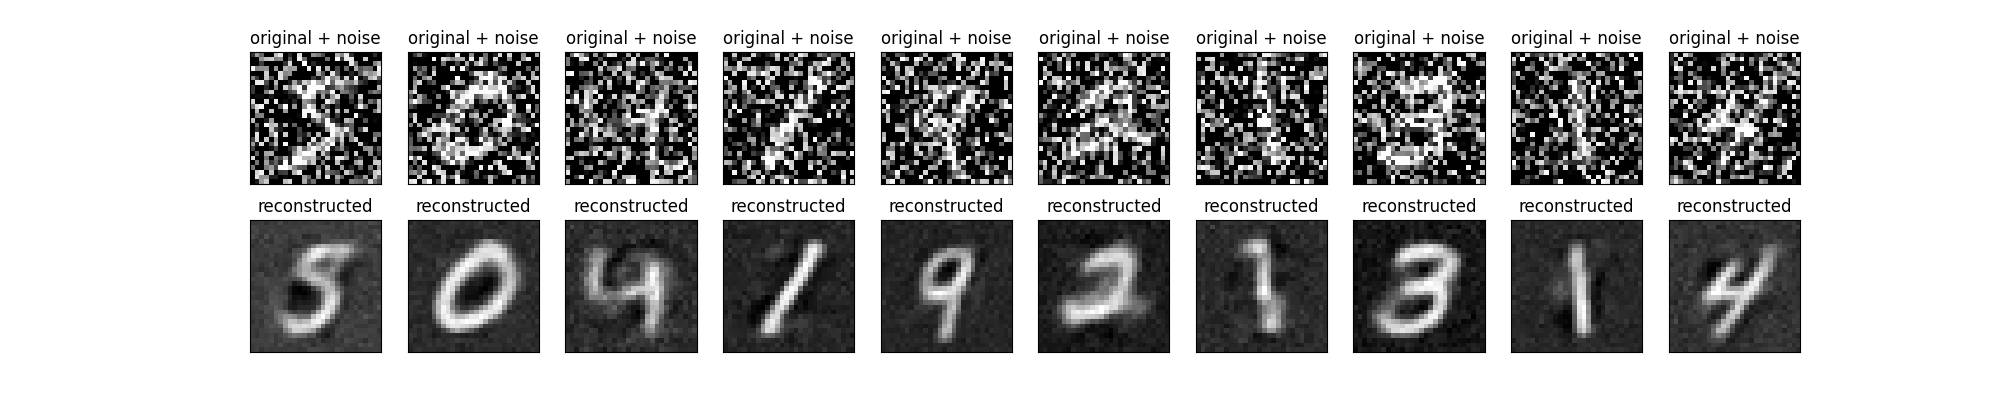
\includegraphics[width=0.95\linewidth]{Images/lam20.0corr0.5/RAE_recon.png}
		\caption[]{RAE cleaned data, corruption $50\%$}
	\end{figure}
\end{frame}

\begin{frame}
	\frametitle{$l_{2,1}$ Robust Deep Autoencoder}
	\begin{itemize}
		\item To assess the performance of RDAE in anomaly detection we start by using a synthetic labeled dataset.
		\item All the $4$ digit images for training are collected in our dataset.
		\item Then, some images are chosen at random from all the other digits until they reach $5\%$ of total images in the dataset.
		\item These will be considered as the outliers of our data.
	\end{itemize}
\end{frame}


\begin{frame}
	\begin{itemize}
		\item The $l_{2,1}$ RDAE is trained on this dataset without any side information. It has to recognize outliers completely on its own. Same architecture as before.
		\item The only parameter that requires tuning is $\lambda$. We assess performance with the accuracy, precision, recall and $F1=2\frac{PR}{P+R}$ metrics.
		\item We consider an instance anomalous whenever the $S$ matrix has non-zero entries on its row.
	\end{itemize}
\end{frame}

\begin{frame}
	\frametitle{Anomaly detection performance}
	\begin{figure}
		\centering
		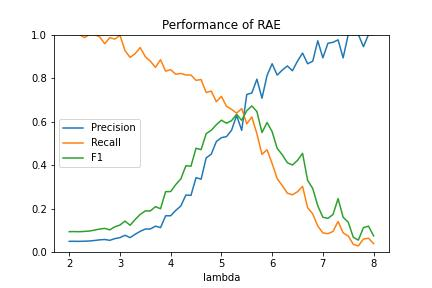
\includegraphics[width=0.8\linewidth]{Images/l21_experiment_from_0.1_to_10.1.jpg}
		\caption[]{$L_{2,1}$ RDAE anomaly detection performance. $\lambda$ from $2$ to $8$}
	\end{figure}
\end{frame}

\begin{frame}
	\begin{itemize}
		\item The maximum performance is obtained with $\lambda=5.468$ with an $F_1$ score of $0.668$.
		\item Focusing on all values from $\lambda=5$ to $\lambda=6$ the RDAE has a $F_1$ score almost everytime above $0.55$.
		\item Precision and recall are both in the range $[0.6, 0.7]$ for $\lambda$ close to the optimal.
		\item Let's look at the reconstructions by the DAE of the RDAE $D(E(X))$, the cleaned images $L_D$ and the sparse image $S$ from $3$ different values of $\lambda$: low, optimal and high.
	\end{itemize}
\end{frame}

\begin{frame}
	\frametitle{Original Images data}
	\begin{figure}
		\centering
		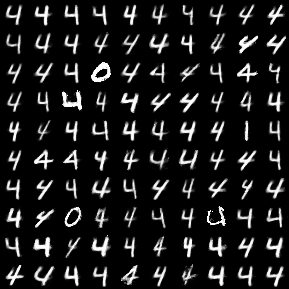
\includegraphics[width=0.5\linewidth]{Images/original_l21.png}
		\caption[]{Original images for the $L_{2,1}$ RDAE}
	\end{figure}
\end{frame}

\begin{frame}
	\frametitle{$\lambda=5.468$}
	\begin{figure}
		\centering
		\begin{subfigure}[b]{0.3\textwidth}
			\centering
			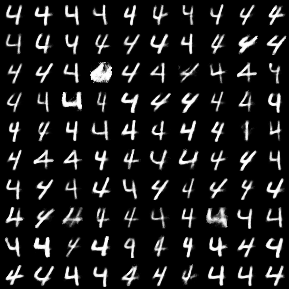
\includegraphics[width=\textwidth]{Images/l21R_5.468.png}
			\caption{$\bar{X}$, reconstruction}
		\end{subfigure}
		\hfill
		\begin{subfigure}[b]{0.3\textwidth}
			\centering
			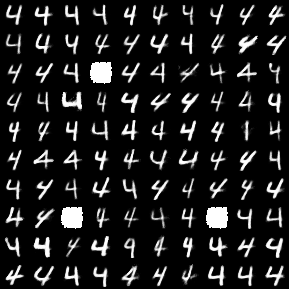
\includegraphics[width=\textwidth]{Images/l21L_5.468.png}
			\caption{$L_D$, cleaned data}
		\end{subfigure}
		\hfill
		\begin{subfigure}[b]{0.3\textwidth}
			\centering
			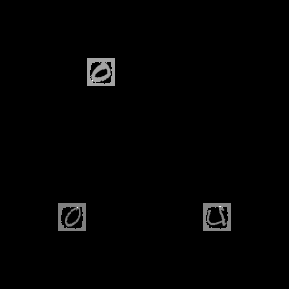
\includegraphics[width=\textwidth]{Images/l21S_5.468.png}
			\caption{$S$, outliers}
		\end{subfigure}
		   \caption{Accuracy: $0.970$, precision: $0.722$, recall: $0.621$, F1 score: $0.668$}
   \end{figure}
\end{frame}

\begin{frame}
	\frametitle{$\lambda=8.0$}
	\begin{figure}
		\centering
		\begin{subfigure}[b]{0.3\textwidth}
			\centering
			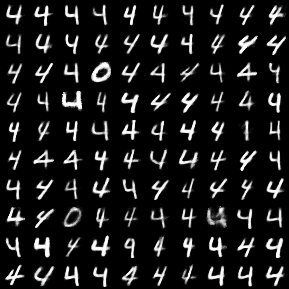
\includegraphics[width=\textwidth]{Images/l21R_8.png}
			\caption{$\bar{X}$, reconstruction}
		\end{subfigure}
		\hfill
		\begin{subfigure}[b]{0.3\textwidth}
			\centering
			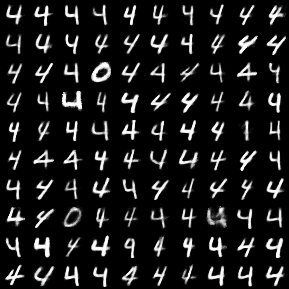
\includegraphics[width=\textwidth]{Images/l21L_8.png}
			\caption{$L_D$, cleaned data}
		\end{subfigure}
		\hfill
		\begin{subfigure}[b]{0.3\textwidth}
			\centering
			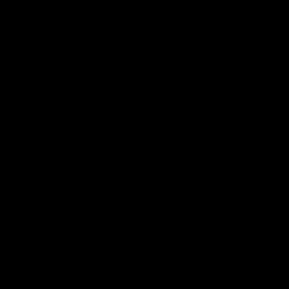
\includegraphics[width=\textwidth]{Images/l21S_8.png}
			\caption{$S$, outliers}
		\end{subfigure}
		   \caption{Accuracy: $0.953$, precision: $1.00$, recall: $0.0386$, F1 score: $0.0743$}
   \end{figure}
\end{frame}

\begin{frame}
	\frametitle{$\lambda=4.0$}
	\begin{figure}
		\centering
		\begin{subfigure}[b]{0.3\textwidth}
			\centering
			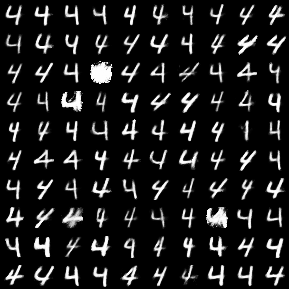
\includegraphics[width=\textwidth]{Images/l21R_4.png}
			\caption{$\bar{X}$, reconstruction}
		\end{subfigure}
		\hfill
		\begin{subfigure}[b]{0.3\textwidth}
			\centering
			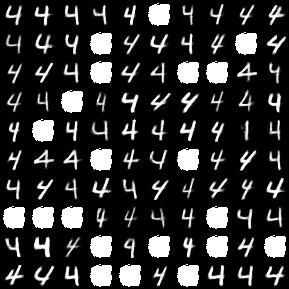
\includegraphics[width=\textwidth]{Images/l21L_4.png}
			\caption{$L_D$, cleaned data}
		\end{subfigure}
		\hfill
		\begin{subfigure}[b]{0.3\textwidth}
			\centering
			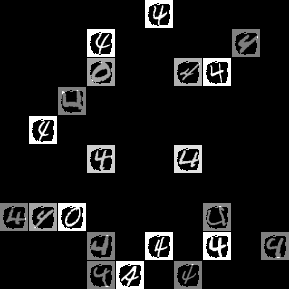
\includegraphics[width=\textwidth]{Images/l21S_4.png}
			\caption{$S$, outliers}
		\end{subfigure}
		   \caption{Accuracy: $0.788$, precision: $0.167$, recall: $0.839$, F1 score: $0.278$}
   \end{figure}
\end{frame}

\begin{frame}
	\begin{itemize}
		\item The performance of the RDAE as outlied detector is compared with the one obtained using the isolation forest method.
		\item The isolation forest method it is based on the idea that outliers are few and very different from the rest.
		\item These outliers gets recognized using isolation trees which try to separate points from others.
		\item The only parameter to be optimized is the outlier fraction (from $0$ to $0.5$).
	\end{itemize}
\end{frame}

\begin{frame}
	\frametitle{Isolation forest performance}
	\begin{figure}
		\centering
		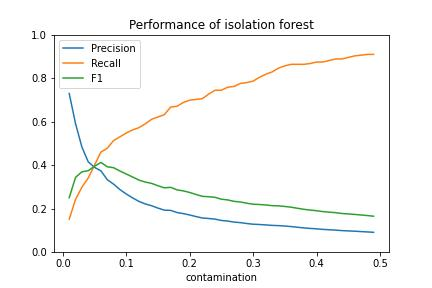
\includegraphics[width=0.8\linewidth]{Images/isolation_forest.jpg}
		\caption[]{The performance is far worse than RDAE.}
	\end{figure}
\end{frame}

\begin{frame}
    \frametitle{Real World Experiment}
    \begin{itemize}
        \item Now we have assessed the performance on a synthetic dataset we want to see how to apply this model to real world challenges.
        \item Data is in general UNLABELED. Specially with loads of data, we can't do hand labeling of anomalies.
        \item We want to see if the model still works for time series.
        \item This could have a true application in Electra Vehicles products: given historical battery data if we are able to detect anomalies we can better spot dangers and errors.
    \end{itemize}
\end{frame}

\begin{frame}
	\frametitle{Time series experiment}
	\begin{itemize}
		\item In this case we are going to use a dataset similar to our interest.
        \item It is taken from the Numenta Anomaly Benchmark \hyperref{https://github.com/numenta/NAB/tree/master/data}{}{}{(NAB)}. The database is called machine temperature system failure.
		\item It is the sensor data of an internal component of a large, industrial mahcine. It should have $3$ kinds of anomalies: the first anomaly is a planned shutdown of the machine. The second anomaly should be difficult to detect and directly led to the third anomaly, a catastrophic failure of the machine.
	\end{itemize}
\end{frame}

\begin{frame}
    \frametitle{Data processing pipeline}
    \begin{itemize}
        \item Data has $22464$ timesteps in total. Data signals are taken every $5$ minutes.
        \item I chose to consider subsequences of length $144$: this corresponds of windows of $12$ hours. The final dataset has then $22321$ training time series.
		\item Data is normalized all togheter to be in $(0,1)$.
    \end{itemize}
\end{frame}

\begin{frame}
	\frametitle{RDAE architectures and analysis}
	I tried using $3$ architectures for the autoencoder part in the RDAE.
	\begin{itemize}
		\item The first one is a Dense Neural Network with hidden layers of $60$ and $20$. It is trained for $20$ outer iterations and $50$ inner iterations for the autoencoder, batch size $256$ , $\epsilon=10^{-8}$.
		\item The second and the third one are a LSTM and a GRU with two layers of $32$ and $16$ units, $10$ outer iterations and $25$ inner iterations with same batch size as before.
		\item Since data is unlabeled we don't have a clear benchmark for the valie of $\lambda$. I tried different values to see how the number of outliers scales.
	\end{itemize}
\end{frame}

\begin{frame}
	\frametitle{Anomalies found}
	\begin{table}[width=\linewidth]
		\begin{tabular}{|c|c|c|c|c|c|c|c|c|c|}
		\hline
		\textbf{$\lambda$} & \textbf{$0.1$} & \textbf{$0.5$} & \textbf{$0.7$} & \textbf{$1.0$}  & \textbf{$2.0$} & \textbf{$3.0$} & \textbf{$3.2$} & \textbf{$3.3$} & \textbf{$4$}\\ \hline
		\textbf{Dense} & All       & $751$          & $250$          & $14$     & $0$            & $0$            & $0$            & $0$            & $0$ \\ \hline
		\textbf{LSTM}  & All        & $7525$         & $4208$         & $2068$  & $306$          & $109$          & $74$           & $9$            & $0$ \\ \hline
		\textbf{GRU}  & All        & $7277$         & $4505$         & $2454$  & $331$          & $139$          & $103$           & $80$            & $0$ \\ \hline
		\end{tabular}
		\caption[]{Anomalies found by the two architecures w.r.t. $\lambda$}
	\end{table}
\end{frame}

\begin{frame}
	\frametitle{Dense RDAE}
	\begin{figure}
		\centering
		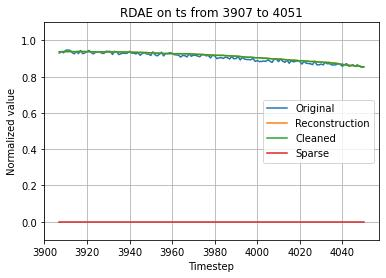
\includegraphics[width=0.7\linewidth]{Images/lam1.0ts_non_anomaly3907.jpg}
		\caption[]{Example of a non anomaly subsequence for $\lambda=1.0$}
	\end{figure}
\end{frame}

\begin{frame}
	\frametitle{Dense RDAE}
	\begin{figure}
		\centering
		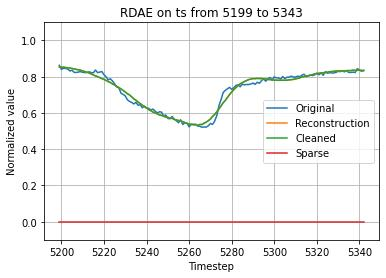
\includegraphics[width=0.7\linewidth]{Images/lam1.0ts_non_anomaly5199.jpg}
		\caption[]{Example of a non anomaly subsequence for $\lambda=1.0$}
	\end{figure}
\end{frame}

\begin{frame}
	\frametitle{Dense RDAE}
	\begin{figure}
		\centering
		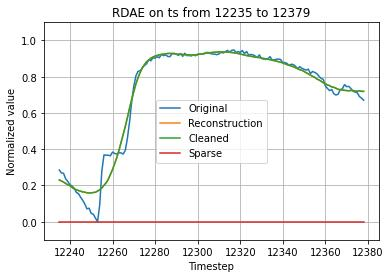
\includegraphics[width=0.7\linewidth]{Images/lam1.0ts_non_anomaly12235.jpg}
		\caption[]{Example of a non anomaly subsequence for $\lambda=1.0$}
	\end{figure}
\end{frame}

\begin{frame}
	\frametitle{Dense RDAE}
	\begin{figure}
		\centering
		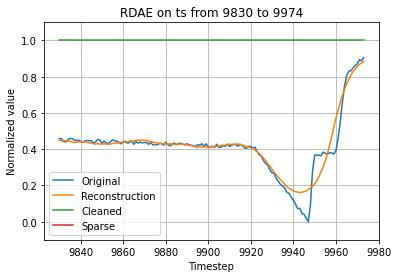
\includegraphics[width=0.7\linewidth]{Images/lam1.0ts_anomalyzoom9830.jpg}
		\caption[]{Example of a anomaly subsequence for $\lambda=1.0$}
	\end{figure}
\end{frame}

\begin{frame}
	\frametitle{Dense RDAE}
	\begin{figure}
		\centering
		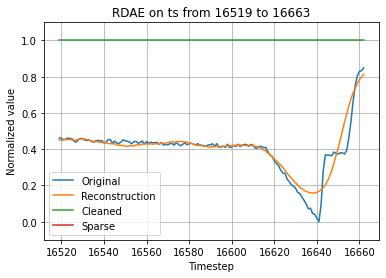
\includegraphics[width=0.7\linewidth]{Images/lam1.0ts_anomalyzoom16519.jpg}
		\caption[]{Example of a anomaly subsequence for $\lambda=1.0$}
	\end{figure}
\end{frame}

\begin{frame}
	\frametitle{Dense RDAE}
	\begin{figure}
		\centering
		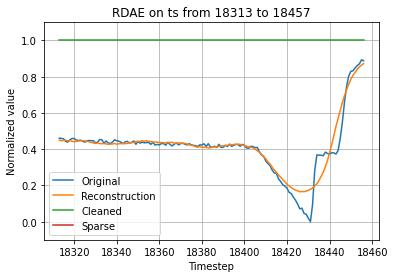
\includegraphics[width=0.7\linewidth]{Images/lam1.0ts_anomalyzoom18313.jpg}
		\caption[]{Example of a anomaly subsequence for $\lambda=1.0$}
	\end{figure}
\end{frame}

\begin{frame}
	\frametitle{Dense RDAE}
	\begin{itemize}
		\item All of the anomalies found reach the $0$ value (min temperature of all time series).
		\item Note that the different anomalies found DO NOT overlap. So each of the failures is only recognized once.
		\item This may also create problems, since as you can see one failure is not recognized as anomaly.
		\item In general, the reconstruction is a non-noisy version of the signal.
	\end{itemize}
\end{frame}

\begin{frame}
	\frametitle{LSTM RDAE}
	\begin{figure}
		\centering
		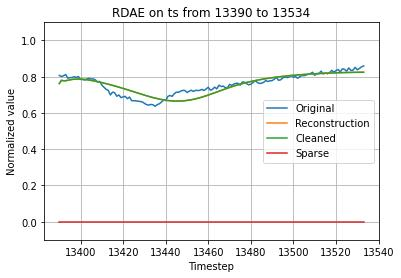
\includegraphics[width=0.7\linewidth]{Images/LSTMlam3.3ts_non_anomaly13390.jpg}
		\caption[]{Example of a non anomaly subsequence for $\lambda=3.3$}
	\end{figure}
\end{frame}


\begin{frame}
	\frametitle{LSTM RDAE}
	\begin{figure}
		\centering
		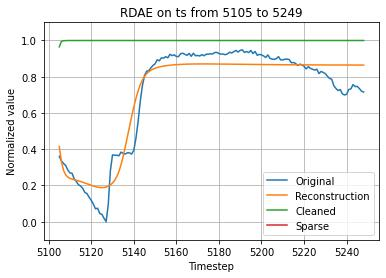
\includegraphics[width=0.7\linewidth]{Images/LSTMlam3.3ts_anomalyzoom5105.jpg}
		\caption[]{Example of a anomaly subsequence for $\lambda=3.3$}
	\end{figure}
\end{frame}

\begin{frame}
	\frametitle{Isolation Forest}
	\begin{itemize}
		\item I tried to fit an isolation forest on the same data, to see if we get the same kind of outliers.
		\item With all outlier fraction values tested ($0.0001, 0.0005, 0.001, 0.01$), non of them showed significant results.
		\item On the contrary, almost all the anomalies detected I saw were normal time series, almost flat.
	\end{itemize}
\end{frame}

\begin{frame}
	\frametitle{Isolation forest anomaly example}
	\begin{figure}
		\centering
		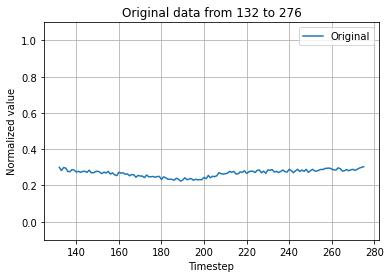
\includegraphics[width=0.7\linewidth]{Images/anom_if0.001pos132.jpg}
		\caption[]{Example of an anomaly found by the isolation forest with outlier fraction of $0.001$}
	\end{figure}
\end{frame}

\begin{frame}
	\frametitle{Final comments}
	\begin{itemize}
		\item The RDAE is a powerful tool for denoising and anomaly detection.
		\item Unfortunately the main quest is to find the correct $\lambda$ value. With unlabeled data this could be very difficult.
		\item In that case, a possible way out is to know the approximate anomaly rate and to hope the anomalies found match the true ones.
	\end{itemize}
\end{frame}

\begin{frame}
	\begin{itemize}
		\item Note an important thing: after we train the model where is no way to find anomalies on new given data.
		\item The $L_D$ and $S$ matrices are produced only in the training procedure.
		\item We can still denoise images with the Autoencoder part.
		\item It could be tried to add new data after some iteration, without re-initializing. This requires training again the autoencoder, which is the high computational part.
	\end{itemize}
\end{frame}

\begin{frame}
\centering{\hyperref{https://github.com/AlexThirty/SaMLMfTSA}{}{}{https://github.com/AlexThirty/SaMLMfTSA}}
	\Huge{\centerline{Thank you!}} 
\end{frame}

\nocite{RAE}
\nocite{DATA}
\nocite{RPCA}
\nocite{PROX}

\bibliographystyle{alpha}
\bibliography{Bibliography}



%----------------------------------------------------------------------------------------

\end{document}
